\documentclass{amsart}
\usepackage[usefamily=sage]{pythontex} 
%\usepackage{sagetex} 
\usepackage{float}
\usepackage{tikz}
\usetikzlibrary{calc}
\usepackage[utf8]{inputenc}
\usepackage[most]{tcolorbox}
\usepackage[margin = 2cm]{geometry}

\newtheorem{ejer}{Ejercicio}
\def\r{\mathbb{R}}
\title{Tarea 08. Giros en el Plano \\ AMD 2023-24}

\begin{document}
\maketitle

\begin{ejer}
Construye la bandera de Chile con la especificaciones indicadas el el siguiente gráfico:

\begin{figure}[H]
\centering
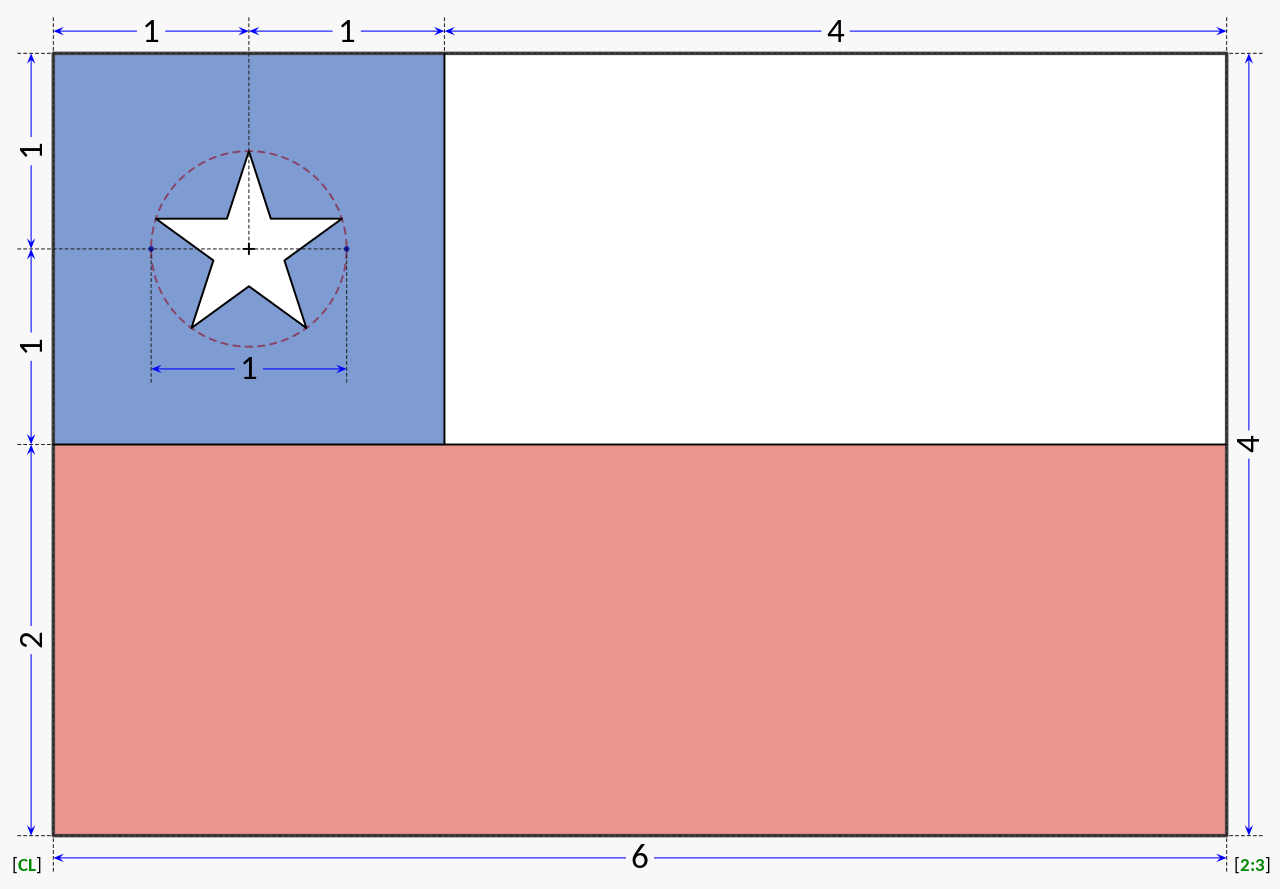
\includegraphics[width = 12cm]{Chile.png}
%(Fuente: \url{https://en.wikipedia.org/wiki/Flag_of_Chile#/media/File:Flag_of_Chile_(construction_sheet).svg})
\end{figure}
\end{ejer}

{\it Solución:}

% Escribe tu solución para el ejercicio 4

\begin{sageblock}
beta = 2*pi/5
r = 0.5
RM = matrix(RR, [[cos(beta), -sin(beta)], [sin(beta), cos(beta)]])

V = [(RM^i * vector([0, 1]) * r) + vector([1, 3]) for i in range(5)]
\end{sageblock}

$$
\sage{V}
$$

\begin{sagesub}
\begin{tikzpicture}
\fill[color = blue] (0, 2) -- (0, 4) -- (2, 4) -- (2, 2);
\fill[color = white] (2, 2) -- (2, 4) -- (6, 4) -- (6, 2);
\fill[color = red] (0, 0) -- (6, 0) -- (6, 2) -- (0, 2);

\fill[color = white] !{V[0]} -- !{V[3]} -- !{V[1]} -- !{V[4]} -- !{V[2]} -- !{V[0]} -- cycle;
\end{tikzpicture}
\end{sagesub}

\end{document}
